\documentclass[10pt]{beamer}
%\documentclass[10pt, handout]{beamer}
%\setbeameroption{show notes}

%\documentclass[10pt, a4paper]{article}
%\usepackage{beamerarticle}




\mode<article>{
	
	\usepackage{hyperref}
	
}
\mode<presentation>{
	
	\usetheme{Antibes}
	\usefonttheme{professionalfonts} 
	\usefonttheme{serif} % default family is serif
	
	%\usecolortheme{spruce} %зеленая, плохой цвет в заголовках 
	%\usecolortheme{albatross} %синяя, пхоло виден черный цвет
	
}

\newcommand{\MP}[1]{\mode<presentation>{#1} }
\newcommand{\MA}[1]{\mode<article>{#1} }

\newcommand{\ABS}[1]{\left| #1 \right|}
%\newcommand{\ABS}[1]{\mid #1 \mid}

\newcommand{\HREF}[2]{{\color{blue}\underline{\href{#1}{#2}}}}

\setbeamertemplate{caption}[numbered]


%\usepackage[T2A]{fontenc}
%\usepackage[utf8]{inputenc}
%\usepackage[russian]{babel}
%\usepackage{amsmath} %математические формулы



\usepackage{ifthen}

\usepackage{tikz}
\usetikzlibrary{arrows.meta}

\usepackage{fp}
\usepackage{tikz-3dplot}
\usepackage{environ}
\usepackage{animate}




\usepackage{xcolor}
%\usepackage[left=20mm,right=20mm,top=20mm,bottom=20mm,a4paper]{geometry} %поля

\usepackage{amsmath} %математические формулы


\usepackage[e]{esvect}  %Красивая стрелочка вектора
%\let\oldvv\vv
\newcommand{\VV}[1]{\vv{#1\mathstrut}}



\usepackage{graphicx} %работа с каритнками


\usepackage{multimedia}

%Для XeLatex/+
\usepackage{polyglossia}
\setdefaultlanguage{russian}
\setotherlanguage{english}
\setkeys{russian}{babelshorthands=true}


\usepackage{fontspec}

\setmainfont{Times New Roman} [Script=Cyrillic, Mapping=tex-text,]
\setsansfont{Arial} [Script=Cyrillic, Mapping=tex-text,]
\setmonofont{Courier New} [Script=Cyrillic, Mapping=tex-text,]



\usepackage{unicode-math}
%\setmathfont{TeX Gyre Termes Math}

%\setmainfont{CMU Serif}[Script=Cyrillic, Mapping=tex-text,]
%\setsansfont{CMU Sans Serif}[Script=Cyrillic, Mapping=tex-text,]
%\setmonofont{CMU Typewriter Text}[Script=Cyrillic, Mapping=tex-text,]


%-----------------


%\usepackage{caption}
%\DeclareCaptionLabelSeparator{dot}{~---~}            %Разделитель номер рисунка
%\captionsetup[figure]{justification=centering,labelsep=dot, format=plain}                        %Подпись рис. центр
%\captionsetup[table]{justification=raggedleft,labelsep=dot, format=plain, singlelinecheck=false} %Подпись табл. слева
%\captionsetup[lstlisting]{justification=raggedleft,labelsep=dot, format=plain, singlelinecheck=false}                     %Подпись рис. центр

\usepackage{indentfirst} %отступ первой строки


\usepackage[svgnames]{xcolor}


%\usepackage{showframe}


%\usepackage{tikz}

%\usepackage[hidelinks]{hyperref}%ссылки внутри документа \ref


\setlength\abovecaptionskip{-2pt}
%\setlength\belowcaptionskip{-14pt}

\setbeamerfont{caption}{size=\scriptsize}


\def\sectionname{Раздел}
\def\subsectionname{Подраздел}


\newcommand{\TC}[3]
{
	
	
	\begin{columns}
		\begin{column}{#1\textwidth}
			#2
		\end{column}
		\begin{column}{\fpeval{1-#1}\textwidth}
			#3
		\end{column}
	\end{columns}
}

\newcommand{\TCT}[3]
{
	
	\begin{columns}[T]
		\begin{column}{#1\textwidth}
			#2
		\end{column}
		\begin{column}{\fpeval{1-#1}\textwidth}
			#3
		\end{column}
	\end{columns}
}


\newcommand{\FRAME}[2]{
	\begin{frame}
		\frametitle{#1}
		#2
	\end{frame}
}

\newcommand{\FIG}[3]
{
	\begin{figure}
		\centering
		\includegraphics[width=#3]{#1}
		\caption{#2}
	\end{figure}
}

\newcommand{\vect}[1]{\overrightarrow{#1}}


\usepackage{newfile}

\edef\LectionNumber{0}

\let\oldsection\section
\let\oldsubsection\subsection


\AtBeginDocument
{
	\newoutputstream{CONTENT}
	\openoutputfile{\LectionNumber .gvr}{CONTENT}
	
	\expandafter\addtostream{CONTENT}{\noindent\textbf{\Large\inserttitle}\unexpanded{\setcounter{SEC}{0}}\par}
}

\renewcommand{\section}[1]{
	\oldsection{#1}
	\expandafter\addtostream{CONTENT}{\noindent\hspace{2ex}\unexpanded{\hbox{\large\stepcounter{SEC}\theSEC ~ #1}}\par}
}

\renewcommand{\subsection}[1]{
	\oldsubsection{#1}
	\expandafter\addtostream{CONTENT}{\noindent\hspace{6ex}\unexpanded{\stepcounter{SUB}\theSUB ~ #1}\par}
}

%\renewcommand{\section}[1]{\MMM{#1}}

%\edef\subsection#1
{
	%\noexpand\subsection{#1}
	%
}


\author{Гаврилов Андрей Геннадьевич}
\institute{Кафедра Информационных технологий и вычислительных систем \\МГТУ~<<СТАНКИН>>}
\lecture{История компьютерной графики}{kghistory}\subtitle{Компьютерная графика}



\graphicspath{{Images/}{Images/L4}}

\date{\today}


\renewcommand{\LectionNumber}{4}
\title{Лекция 4 \\Преобразования точек в пространстве}


\usepackage{standalone}

\setbeamersize
{
	text margin left=0.5cm,
	text margin right=0.5cm
}

\usepackage{comment}


%	\transduration{2}
%   \transfade

 \begin{document}
 		 
	\makeatletter
\defbeamertemplate*{title page}{my theme}
{
	
	\hfill
	
	\begin{beamercolorbox}[wd=.9\paperwidth,center,]{title}%
		
	\end{beamercolorbox}%	
	
	\vbox to 1em {}
	
	\begin{beamercolorbox}[wd=.9\paperwidth,center,]{title}%
		\usebeamerfont{subtitle}%
		\hfill
		
		\insertsubtitle
		
		\usebeamerfont{title}%
		\inserttitle{} \\[0.5em]
		
		
		
	\end{beamercolorbox}%	
	\hfill\hfill
	
	\begin{beamercolorbox}[wd=.9\paperwidth,center,]{}%
		\usebeamerfont{author}%
		\hfill \\[0.5em]
		\insertauthor{}
		
		\vbox to 1em{}
		\usebeamerfont{institute}%
		\insertinstitute {}
		
		\vbox to 1em{}			
		{\; }\insertshortdate{}
		
	\end{beamercolorbox}%	
	\hfill\hfill
	
	\vbox to 5em{}
	
	
}
\defbeamertemplate*{footline}{my theme}{
	\leavevmode%
	\hbox{%
		\begin{beamercolorbox}[wd=.25\paperwidth,ht=2.25ex,dp=1ex,center]{author in head/foot}%
			\usebeamerfont{author in head/foot}%
			\insertauthor~~\beamer@ifempty{\insertshortinstitute}{}
		\end{beamercolorbox}%
		\begin{beamercolorbox}[wd=.65\paperwidth,ht=2.25ex,dp=1ex,center]{title in head/foot}%
			\usebeamerfont{title in head/foot}\insertshortinstitute
		\end{beamercolorbox}%
		\begin{beamercolorbox}[wd=.1\paperwidth,ht=2.25ex,dp=1ex,right]{date in head/foot}%
			\usebeamerfont{date in head/foot}\hspace*{2em}
			\insertframenumber{} / \inserttotalframenumber\hspace*{2ex}
	\end{beamercolorbox}}%
}



\makeatother






%float page top aligment
\makeatletter
\setlength{\@fptop}{0pt}
\setlength{\@fpbot}{0pt plus 1fil}
\makeatother

\begin{comment}

\end{comment}

    
    \begin{frame}[plain]
    	
    	
    	\centering
    	Трансляция презентации (во время очных лекций).     
    		
    	
\includegraphics[width=0.5\textwidth, keepaspectratio]{qr.png} \\ ~ \\
    	
    	
    	При просмотре презентации в PDF для отображения анимаций на слайдах необходимо использовать Acrobat Reader, KDE Okular, PDF-XChange или Foxit Reader.

    \end{frame}
	
	
	\frame{\maketitle}
	
	
	
	\begin{frame}{План лекции}
		\tableofcontents
	\end{frame}
	
	
	
	\section{Матрица преобразований}
	
	\frame{\sectionpage}
	
	\begin{frame}{Матрица преобразований}
		
		\TCT{0.5}
		{
			$   \left(
			\begin{array}{ccc|c}
				a & b & c & k \\
				d & e & f & l \\
				g & h & i & m \\ \hline
				o & p & q & r \\				
			\end{array}
			\right) = 
			\left(
			\begin{array}{c|c}
				\textbf M_{11} & \textbf M_{12} \\ \hline
                \textbf M_{21} & \textbf M_{22}						
			\end{array}
			\right)
			$
		}
		{
			$\textbf M_{11}$  --- линейное преобразование \footnotemark 
				
			$\textbf M_{12}$ --- перемещение 
			
			$\textbf M_{21}$ --- перспективное преобразование
			
			$\textbf M_{22}$ --- общее масштабирование
		} 
		
		\footnotetext[1]{Линейное преобразование ---
			это преобразование, переводящее линейную комбинацию векторов в ту же самую линейную комбинацию преобразованных векторов. \\ ~}
		
		\hfil \\ ~ \\

		\pause
		
		$
		\left(
		\begin{array}{cccc}
			a & b & c & k \\
			d & e & f & l \\
			g & h & i & m \\ 
			o & p & q & r \\				
		\end{array}
		\right)
		\begin{pmatrix}
			wx\\wy\\wz\\w
		\end{pmatrix}
		=
		\begin{pmatrix}
			awx+bwy+cwz+kw\\
			dwx+ewy+fwz+lw\\
			gwx+hwy+lwz+mw\\
			owx+pwy+qwz+rw\\
		\end{pmatrix}
	   \Rightarrow
		$\\
		$
		\Rightarrow
		\begin{pmatrix}
			(ax+by+cz+k)/(ox+py+qz+r)\\
			(dx+ey+fz+l)/(ox+py+qz+r)\\
			(gx+hy+lz+m)/(ox+py+qz+r)\\
			1\\
		\end{pmatrix}
		$
		
		 
	\end{frame}
	
    
    \section{Аффинные преобразования}
    
    \frame{\sectionpage}
    
    \subsection{Перенос объекта}

	\begin{frame}{Перенос}
		
		\TC{0.5}
		{
			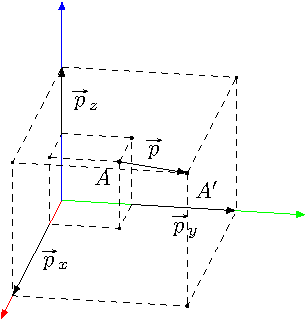
\includegraphics{trans.pdf}
		}
		{
			\begin{block}{Матрица переноса}
				$$
				\textbf{T}(\vv p) =
				\begin{pmatrix}
					1 & 0 & 0 & p_x\\
					0 & 1 & 0 & p_y\\
					0 & 0 & 1 & p_z\\
					0 & 0 & 0 & 1\\
				\end{pmatrix}
				$$
			\end{block}
			$\textbf{T}(\vv p)\textbf{A}=\textbf{A}'$ \\[0.5em]
			$
			\begin{pmatrix}
				1 & 0 & 0 & p_x\\
				0 & 1 & 0 & p_y\\
				0 & 0 & 1 & p_z\\
				0 & 0 & 0 & 1\\
			\end{pmatrix}
			\begin{pmatrix}
				x\\
				y\\
				z\\
				1
			\end{pmatrix}
			=
			\begin{pmatrix}
				x+p_x\\
				y+p_y\\
				z+p_z\\
				1
			\end{pmatrix}			
			$
		}
		
	\end{frame}
	
	\begin{frame}{Перенос объекта}
		\TCT{0.45}
		{
			\animategraphics[autoplay,loop]{0.25}{Images/L4/pyrotrans}{0}{4} 
		}
		{
			$\mathbf V = 
			\begin{pmatrix}
				0.5 & -0.5 &-0.5& 0.5& 0\\
				0.5 & 0.5& -0.5& -0.5 & 0\\
				-0.5& -0.5& -0.5 &-0.5& 0.5\\
				1& 1& 1& 1& 1
			\end{pmatrix}$ \\ ~ \\
			
			$\mathbf V' = \mathbf{TV}$
			
			
		}
	\end{frame}

	\subsection{Масштабирование объекта}
	
	
	\begin{frame}{Масштабирование}
		
		\TC{0.45}
		{
			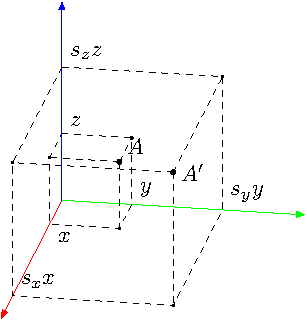
\includegraphics{scale.pdf}
		}
		{
			\begin{block}{Матрица масштабирования}
				$$
				\textbf{S}(\vv s) =
				\begin{pmatrix}
					s_x & 0 & 0 & 0\\
					0 & s_y & 0 & 0\\
					0 & 0 & s_z & 0\\
					0 & 0 & 0 & 1\\
				\end{pmatrix}
				$$
			\end{block}
			
			$\textbf{S}(\vv s)\textbf{A}=\textbf{A}'$ \\[0.5em]
			$
			\begin{pmatrix}
				s_x & 0 & 0 & 0\\
				0 & s_y & 0 & 0\\
				0 & 0 & s_z & 0\\
				0 & 0 & 0 & 1\\
			\end{pmatrix}
			\begin{pmatrix}
				x\\
				y\\
				z\\
				1
			\end{pmatrix}
			=
			\begin{pmatrix}
				s_xx\\
				s_yy\\
				s_zz\\
				1
			\end{pmatrix}			
			$
			
		Если $s_x=s_y=s_z$ масштабирование равномерное.
		}
		
	\end{frame}
	

	\begin{frame}{Масштабирование объекта}
		\TCT{0.45}
		{
			\animategraphics[autoplay,loop]{0.25}{Images/L4/pyroscale}{0}{4} 
		}
		{
			$\mathbf V = 
			\begin{pmatrix}
				0.5 & -0.5 &-0.5& 0.5& 0\\
				0.5 & 0.5& -0.5& -0.5 & 0\\
				-0.5& -0.5& -0.5 &-0.5& 0.5\\
				1& 1& 1& 1& 1
			\end{pmatrix}$ \\ ~ \\
			
			$\mathbf V' = \mathbf{SV}$
			
			
		}
	\end{frame}

	
	\subsection{Поворот объекта}	
	
	\begin{frame}{Повороты}
		\TC{0.5}
		{
			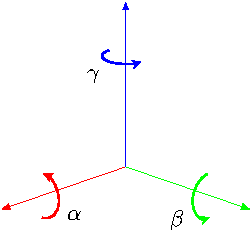
\includegraphics{rotations.pdf}
		}
		{
			\begin{block}{Матрица поворота вокруг $OX$}
				\centering 
				$ R_x(\alpha)
				 =
				 \begin{pmatrix}
				 	1&0&0&0\\
				 	0&\cos\alpha&-\sin\alpha&0\\
				 	0&\sin\alpha&\cos\alpha&0\\
				 	0&0&0&1				 	
				 \end{pmatrix}
				 $				
			\end{block}
			
			
		}
		
		\TC{0.5}
		{
			\begin{block}{Матрица поворота вокруг $OY$}
				\centering 
				$ R_y(\beta)
				=
				\begin{pmatrix}
					\cos\beta&0&\sin\beta&0\\
					0&1&0&0\\
					-\sin\beta&0&\cos\beta &0\\
					0&0&0&1				 	
				\end{pmatrix}
				$				
			\end{block}
		}
		{
				\begin{block}{Матрица поворота вокруг $OZ$}
				\centering 
				$ R_z(\gamma)
				=
				\begin{pmatrix}
					\cos\gamma&-\sin\gamma&0&0\\
					\sin\gamma&\cos\gamma&0&0\\
					0&0&1&0 \\
					0&0&0&1	\\			 	
				\end{pmatrix}
				$				
			\end{block}
		}
	\end{frame}
	
	\begin{frame}{Комбинация поворотов}
		\animategraphics[autoplay,loop]{0.25}{Images/L4/pyrorot}{0}{3} 
		\animategraphics[autoplay,loop]{0.25}{Images/L4/pyrorot2}{0}{3} 
	\end{frame}
	
	\begin{frame}{Поворот вокруг произвольной оси}
		
	
		
				\centering
				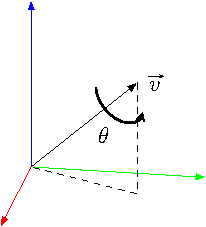
\includegraphics{rotations2.pdf}
				
		
			\begin{block}{Матрица поворота вокруг произвольной оси $\vv v$, $|\vv v| = 1$}
			\footnotesize
			$$
			\mathbf{R}(\vv v, \theta) = 
			\begin{pmatrix}
				\cos \theta + (1 - \cos \theta) x^2
				& (1 - \cos \theta) x y - (\sin \theta) z 
				& (1 - \cos \theta) x z + (\sin \theta) y  
				& 0\\
				(1 - \cos \theta) y x + (\sin \theta) z 
				& \cos \theta + (1 - \cos \theta) y^2
				& (1 - \cos \theta) y z - (\sin \theta) x
				& 0\\
				(1 - \cos \theta) z x - (\sin \theta) y
				& (1 - \cos \theta) z y + (\sin \theta) x
				& \cos \theta + (1 - \cos \theta) z^2 
				& 0 \\
				0 & 0 & 0 & 1
			\end{pmatrix}
			$$
		\end{block}
		
	\end{frame}
	
  \begin{frame}{Поворот объекта вокруг произвольной оси}
  	\TCT{0.5}
  	{
  		\animategraphics[autoplay,loop]{45}{Images/L4/pyrorot3}{0}{359} 
  	}
  	{
  		$\vv v (2,2,2)$ \\ ~ \\
  		
  		$\mathbf V' = \mathbf R\left(\displaystyle\frac{\vv v }{|\vv v|},\theta\right)\mathbf V$
  	}
  	
  \end{frame}
  

\section{Преобразования систем координат}

\frame{\sectionpage}


\begin{frame}{Преобразования систем координат}
	\TC{0.5}
	{
		\only<1>{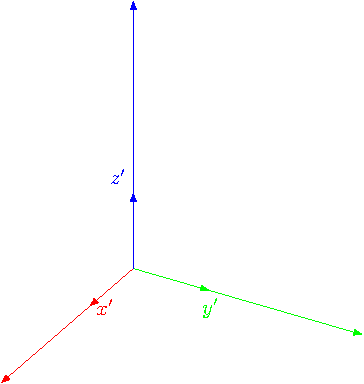
\includegraphics[page=1]{coordsystems.pdf}
		}\only<2>{\includegraphics[page=2]{coordsystems.pdf}
		}\only<3>{\includegraphics[page=3]{coordsystems.pdf}
		}\only<4->{\includegraphics[page=4]{coordsystems.pdf}}
		
	}
	{
		Пусть есть две  совпадающие системы координат (СК) --- $xyz$ (мировая) и $x'y'z'$ (локальная).  \\ ~ \\
				
		\pause 
		
		Преобразуем СК  $x'y'z'$:
		
		\begin{enumerate}
			\item<+-> Повернём на угол $\gamma$ вокруг оси $z$ мировой СК.
			\item<+-> Повернём на угол $\beta$ вокруг оси $y$ мировой СК.
			\item<+-> Перенесём на вектор $\vv t$ относительно начала мировой СК.
		\end{enumerate}
		
		\pause
		
		Запишем эти преобразования в матричной форме:
		
		$\mathbf M = \mathbf T (\vv t) \mathbf R_y (\beta) \mathbf R_z(\gamma)$
	}
\end{frame}

\begin{frame}{Переход между системами координат (простой случай)}
	\TC{0.5}
	{
		\only<1>{\includegraphics[page=5]{coordsystems.pdf}
		}\only<2->{\includegraphics[page=6]{coordsystems.pdf}}
	}
	{
		Рассмотрим 2 СК: мировую $xyz$ и локальную $x'y'z'$, перемещённую на вектор $\vv t$, относительно мировой. \\[0.5em]
		
		Рассмотрим точку $A$ в этих СК: как $A^{xyz}$ и $A^{x'y'z'}$. \\ ~ \\
		
		\pause
		
		$x'y'z' \rightarrow  xyz: \quad {\color{cyan} \vv A^{xyz}} =  {\color{magenta} \vv A^{x'y'z'}} + \vv t $ \\[0.5em]
		$xyz \rightarrow  x'y'z': \quad  {\color{magenta} \vv A^{x'y'z'}}   =  {\color{cyan} \vv A^{xyz}} - \vv t $
		
		
		
		
	}
\end{frame}

\begin{frame}{Переход между системами координат (общий случай)}
	\TC{0.5}
	{
		\includegraphics[page=7]{coordsystems.pdf}
	}
	{
		Рассмотрим 2 СК: мировую $xyz$ и локальную $x'y'z'$, преобразованную относительно мировой матрицей $\mathbf M$. \\[0.5em]
		
		Рассмотрим точку $A$ в этих СК: как $A^{xyz}$ и $A^{x'y'z'}$. \\ ~ \\
		
		\pause
		
		$x'y'z' \rightarrow  xyz: \quad  \mathbf A^{xyz}=\mathbf{M}\mathbf A^{x'y'z'}$ \\[0.5em]
		$xyz \rightarrow  x'y'z': \quad  \mathbf A^{x'y'z'}=\mathbf{M}^{-1}\mathbf A^{xyz}$
		
				
		 
	}
\end{frame}
  

  
  
  \section{Проекционные преобразования}
  \frame{\sectionpage}
  
  
  \subsection{Ортогональная проекция}
  
  \begin{frame}{Ортогональная проекция}
  	\TC{0.4}
  	{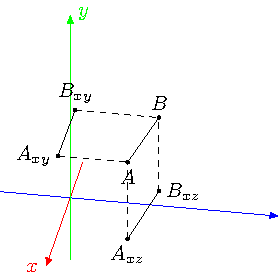
\includegraphics{line_ortho.pdf}
  	}
  	{
  		\begin{block}{Матрицы ортогональной проекции}
  			$$
  			\mathbf P_{xy}=
  			\begin{pmatrix}				
  				1&0&0&0\\
  				0&1&0&0\\
  				0&0&0&0\\
  				0&0&0&1		
  			\end{pmatrix},							
  			\mathbf P_{xz}=
  			\begin{pmatrix}				
  				1&0&0&0\\
  				0&0&0&0\\
  				0&0&1&0\\
  				0&0&0&1		
  			\end{pmatrix}, $$  $$		
  			\mathbf P_{yz}=
  			\begin{pmatrix}				
  				0&0&0&0\\
  				0&1&0&0\\
  				0&0&1&0\\
  				0&0&0&1		
  			\end{pmatrix}		
  			$$
  			
  		\end{block}
  	}
  	
  	\pause
  	
  	$\begin{pmatrix}				
  		1&0&0&0\\
  		0&1&0&0\\
  		0&0&0&0\\
  		0&0&0&1		
  	\end{pmatrix}
  	\begin{pmatrix}
  		wx\\
  		xy\\
  		wz\\
  		w
  	\end{pmatrix}
  	=
  	\begin{pmatrix}
  		wx\\
  		wy\\
  		0\\
  		w\\
  	\end{pmatrix}
  	\Rightarrow
  	\begin{pmatrix}
  		x\\
  		y\\
  		0\\
  		1
  	\end{pmatrix}
  	$
  	
  \end{frame}
  
  
  \subsection{Перспективная проекция}
  

  
  \begin{frame}{Проецирование куба}
  	\TCT{0.5}
  	{
  		\animategraphics[autoplay,loop,viewport=0 0 300 300, width=0.5\framewidth, nomouse]{30}{Images/L4/test}{0}{241} 
  	}
  	{
  		$\textbf{P}=
  		\begin{pmatrix}
  			1&0&0&0\\
  			0&1&0&0\\
  			0&0&1&0\\
  			0&0&1&0
  		\end{pmatrix}$\\~\\
  		Для всех точек куба:\\
  		$ \textbf P \cdot \textbf A =\textbf A'$ \\ ~ \\
  		
  		$
  		\begin{pmatrix}
  			1&0&0&0\\
  			0&1&0&0\\
  			0&0&1&0\\
  			0&0&1&0
  		\end{pmatrix}
  		\begin{pmatrix}
  			wx\\
  			wy\\
  			wz\\
  			w
  		\end{pmatrix}
  		=	
  		\begin{pmatrix}
  			wx\\
  			wy\\
  			wz\\
  			wz
  		\end{pmatrix}
  		= $ \\ 
  		$ \Rightarrow
  		\begin{pmatrix}
  			x/z\\
  			y/z\\
  			1\\
  			1
  		\end{pmatrix}
  		$
  	}
  	
  \end{frame}
  



\begin{frame}{Перспективная проекция}
	
	\centering
	\usetikzlibrary{positioning}
	\begin{tikzpicture}
		
		\node  (img1) {	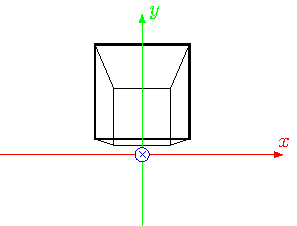
\includegraphics[page=1]{cube perspective.pdf}};
		\node  (img2)  [right = 0 of img1] {  \includegraphics[page=2]{cube perspective.pdf}};
		
		\draw[|->] (3,0.5) -- +(3,0) node [below, midway] {\footnotesize Вид на левое изображение};
		
	\end{tikzpicture}

\end{frame}


  \subsection{Перспективное преобразование}
  
  	\begin{frame}{Матрица перспективного преобразования}
  	\begin{block}{Матрица перспективного преобразования (одна из множества)}
  		$$\mathbf P=\begin{pmatrix}
  			1&0&0&0\\
  			0&1&0&0\\
  			0&0&1&0\\
  			0&0&a&\mathbf{1}
  		\end{pmatrix}$$
  	\end{block}
  	
  	$
  	\begin{pmatrix}
  		1&0&0&0\\
  		0&1&0&0\\
  		0&0&1&0\\
  		0&0&a&1
  	\end{pmatrix}
  	\begin{pmatrix}
  		wx\\
  		wy\\
  		wz\\
  		w
  	\end{pmatrix}
  	=
  	\begin{pmatrix}
  		wx\\
  		wy\\
  		wz\\
  		wza+w
  	\end{pmatrix}
  	\Rightarrow
  	\begin{pmatrix}
  		x / (za+1) \\
  		y / (za+1) \\
  		z  (za + 1) \\
  		1
  	\end{pmatrix}
  	$
  	
  \end{frame}
  

\begin{frame}{Перспективное преобразование}
	\TC{0.65}
	{
		\only<1-3>{\includegraphics[page=30]{line_perspective.pdf}
		}\only<4->{\animategraphics[autoplay, palindrome, nomouse]{30}{Images/L4/line_perspective}{0}{99} }
		
		
	}
	{
		$AB \ \rightarrow \ A'B' \ \rightarrow \ A'_{xy}B'_{xy}$ \\ ~ \\
		
		\pause
		
		$\left(\mathbf{A}'_{xy}\mathbf{B}'_{xy}\right)=\mathbf P_2 \mathbf P_1 \left(\mathbf{AB}\right)$ \ \ \ \footnotemark[1] 	\\ ~ \\
		
		\pause
		
		
		$\mathbf P_1=\begin{pmatrix}
			1&0&0&0\\
			0&1&0&0\\
			0&0&1&0\\
			0&0&a&\mathbf{1}
		\end{pmatrix}$ --- матрица перспективного преобразования.
		
		$\mathbf P_1=\begin{pmatrix}
			1&0&0&0\\
			0&1&0&0\\
			0&0&0&0\\
			0&0&0&1
		\end{pmatrix}$ --- матрица ортографической проекции на $xy$.
		
	}
	
	
		\footnotetext[1]<2->{
			$
			\left(\mathbf{AB}\right) = 
			\begin{pmatrix}
				A_x & A_y & A_z & 1 \\
				B_x & B_y & B_z & 1 
			\end{pmatrix}
			^T
			$ 
			\\ ~ 	 } 
	
\end{frame}





	


\begin{frame}[t]{Перспективное преобразование куба}
		\centering
		\animategraphics[autoplay,loop,viewport=0 0 400 240, width=\textwidth, nomouse]{30}{Images/L4/cube projective true}{0}{241} 

		
\end{frame}


	
\begin{frame}{Перспективное преобразование сцены}	  
	\centering
	\textbf{Исходные объекты}
	
	\animategraphics[autoplay,loop,viewport=0 0 500 400, width=0.6\framewidth, nomouse]{30}{Images/L4/cube projective true multiple}{0}{260} 
\end{frame}

\begin{frame}{Перспективное преобразование сцены}	  
	\centering
	\textbf{Исходные объекты + преобразованные}
	
	\animategraphics[autoplay,loop,viewport=0 0 500 400, width=0.6\framewidth, nomouse]{30}{Images/L4/cube projective true multiple}{261}{522} 
\end{frame}




\begin{frame}{<<Вид из камеры>>}	  
	\centering
	\textbf{Параллельная преобразования проекция на $xy$}
	
	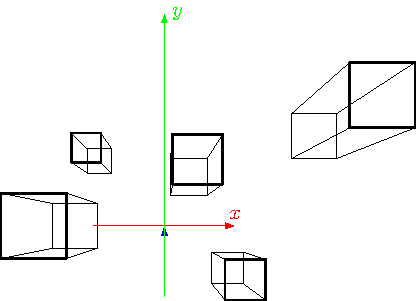
\includegraphics[page=1, width=0.6\textwidth]{cube projective true multiple xy.pdf} 
\end{frame}

\begin{frame}{Двухточечная перспектива}	  
	\centering
	\TC{0.6}
	{
		\includegraphics[page=2, width=\textwidth]{cube projective true multiple xy.pdf} 
	}
	{	
	
			$P = 
			\begin{pmatrix}
				1&0&0&0\\
				0&1&0&0\\	
				0&0&1&0\\	
				0&a&b&1\\		
			\end{pmatrix}$
		
		
	}
	
\end{frame}

\begin{frame}{Трёхточечная перспектива}	  
	\centering
	\TC{0.6}
	{
		\includegraphics[page=3, width=\textwidth]{cube projective true multiple xy.pdf} 
	}
	{	
		
		$P = 
		\begin{pmatrix}
			1&0&0&0\\
			0&1&0&0\\	
			0&0&1&0\\	
			a&b&c&1\\		
		\end{pmatrix}$
		
		
	}
	
\end{frame}


\begin{comment}
\end{comment}

\end{document}